\documentclass[12pt]{presentation}
%\documentclass[compress]{beamer}
\usetheme{default}
%\usecolortheme{whale}
\usepackage{ulem}
\usepackage{amsmath}
\usepackage{url}
\usepackage{graphicx}
\usepackage{pgf}
\usepackage{pgfplots}
\usepackage{tikz}
\usetikzlibrary{fit}					% fitting shapes to coordinates
\usetikzlibrary{backgrounds}	% drawing the background after the foreground
\usetikzlibrary{arrows,automata,calc,patterns,snakes}
\usepackage[latin1]{inputenc}
\usepackage{verbatim}
%Present bigger picture for intro.
%Concrete scenarios
%Clear about defining project: the OUR APPROACH slide!!
%In this particular project Web 2.0 not 1.0 like last time
%Why is this not applicable for threads...
%More data from the collected data...
%Maintain consistent terminologies. `Content-based features'
%HMM must explain more. Time gap.
%how it fits in.
\newcommand{\vocab}{\mathbf{v}}
\newcommand{\dtvec}{\mathbf{t}_\Delta}
\newcommand{\ctxvec}{\mathbf{t}_\text{ctx}}
\newcommand{\dt}{\Delta_t}
\newcommand{\prerror}{Pr_{error}}
\newcommand{\fvec}{\mathbf{X}}
\newcommand{\weights}{\mathbf{w}}
\newcommand{\X}{\mathbf{X}}
\setbeamertemplate{footline}{\insertframenumber/\inserttotalframenumber}
\title{Predicting Web 2.0 Thread Updates\\Progress Update}
\author{Shawn Tan}
\AtBeginSection[]
{
	\begin{frame}{Table of Contents}
	\tableofcontents[currentsection]
	\end{frame}
}
\date{}

\begin{document}
\maketitle
\section{Introduction}

\begin{frame}{Motivation}
	\begin{itemize}
		\item Many sites with thread-based discussion features
		\item Users post product reviews, feedback
	\end{itemize}
	Obtaining such up-to-date information may be vital to companies.
\end{frame}
\section{The Dataset}
\begin{frame}{avsforum.com}
	\begin{center}
		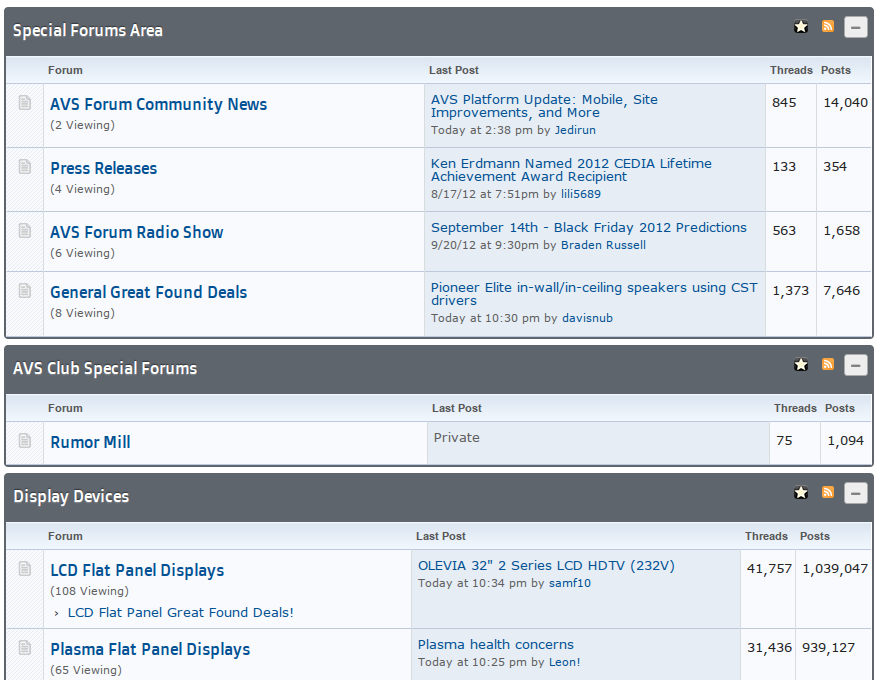
\includegraphics[scale=0.3]{screenshots/index.png}
	\end{center}
\end{frame}

\begin{frame}{User-centric threads}
	\begin{center}
		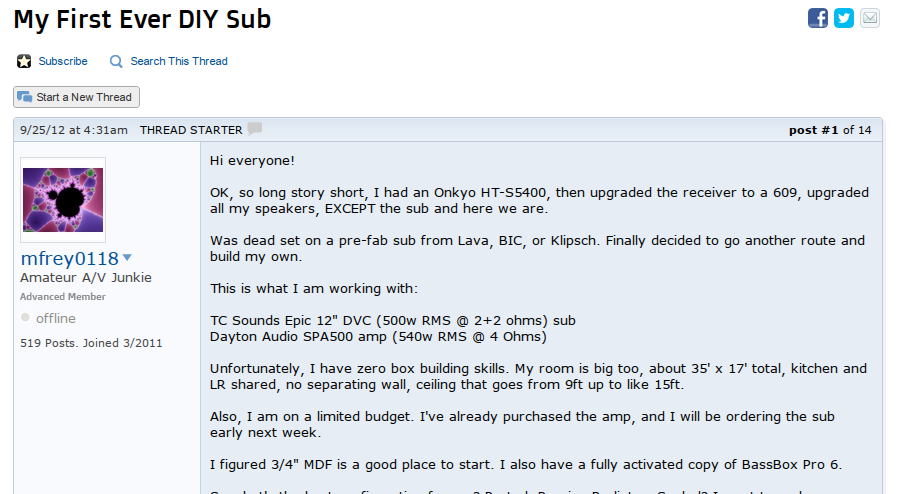
\includegraphics[scale=0.2]{screenshots/revolve_user.png}\\
			$\vdots$\\
		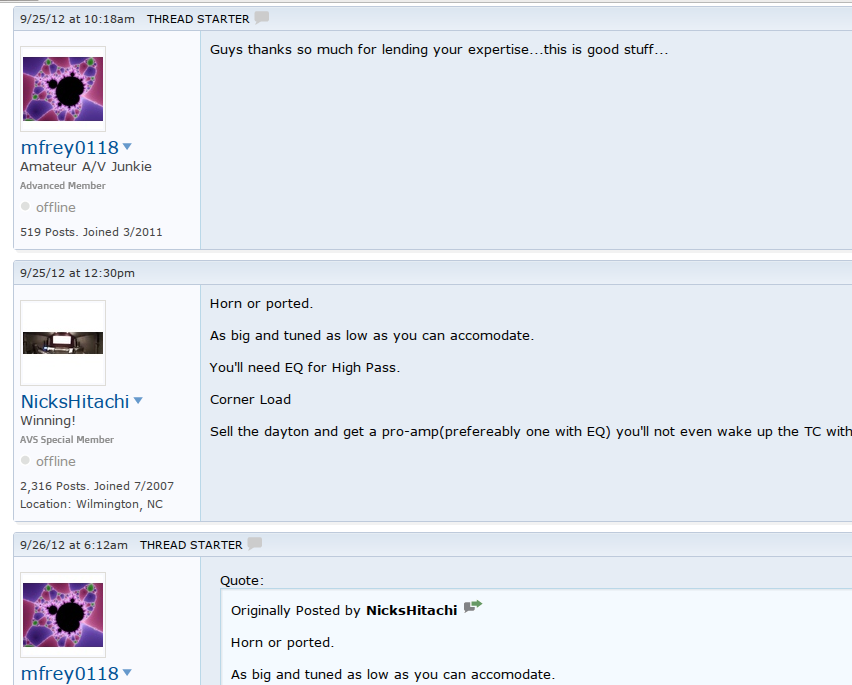
\includegraphics[scale=0.2]{screenshots/revolve_user2.png}
	\end{center}
\end{frame}


\begin{frame}{Questions}
	\begin{center}
		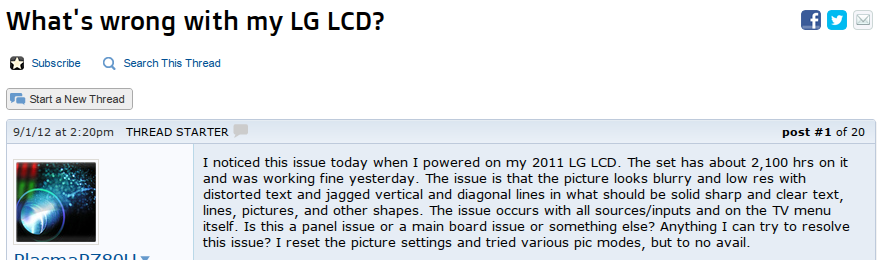
\includegraphics[scale=0.4]{screenshots/question.png}\\
			$\vdots$\\
		
\includegraphics[scale=0.4]{screenshots/question2.png}
	\end{center}
\end{frame}


\begin{frame}{Mentions}
	\begin{center}
		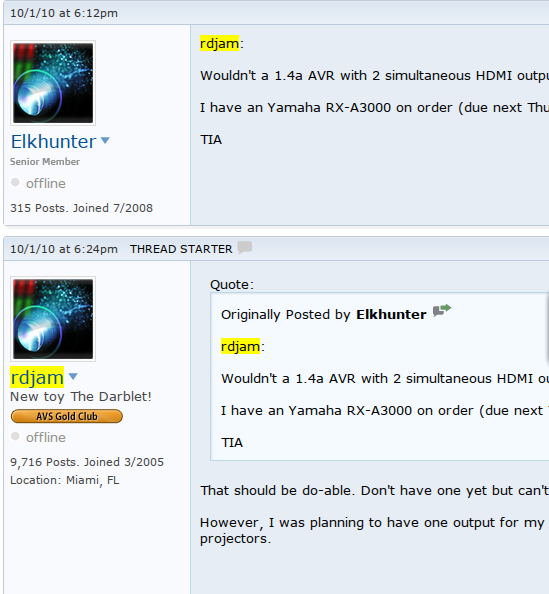
\includegraphics[scale=0.4]{screenshots/replies.png}\\
	\end{center}
\end{frame}


\section{Evaluation Methods}
\begin{frame}{Events}
\begin{center}
	
\tikzstyle{background}=[rectangle,
	fill=gray!10,
	inner sep=0.2cm,
	rounded corners=5mm]


\tikzstyle{post}=[circle,
	thick,
	minimum size=1.2cm,
	draw=blue!80,
	fill=blue!20]
% The measurement vector is represented by an orange circle.
\tikzstyle{visit}=[circle,
	thick,
	minimum size=1.2cm,
	draw=orange!80,
	fill=orange!25]

\begin{tikzpicture}[>=latex,text height=1.5ex,text depth=0.25ex]
    % "text height" and "text depth" are required to vertically
    % align the labels with and without indices.
  
  % The various elements are conveniently placed using a matrix:
  \matrix[column sep=0.3cm] {
    % First line: Control input
    	&
		\node (e0)					{};&
		\node (e1)	[post]			{};&
		\node (e2)	[visit]			{};&
		\node (e3)	[post]			{};&
		\node (e4)	[visit]			{};&
		\node (e5)	[post]			{};&
		\node (e6)	[visit]			{};&
		\node (e)					{};&
		&
        \\
	};
    
    % The diagram elements are now connected through arrows:

	\path[-]
		(e0) edge[thick]	(e1)
		\foreach \e in {1,2,3,4,5}{
			let \n1={int(\e+1)} in (e\e) edge[thick] (e\n1)
		}
		(e6) edge[thick]	(e)
	;

	\begin{pgfonlayer}{background}
		\node [background,fit=(e1) (e3)] {};
	\end{pgfonlayer}

\end{tikzpicture}


\begin{tikzpicture}[>=latex,text height=1.5ex,text depth=0.25ex]
    % "text height" and "text depth" are required to vertically
    % align the labels with and without indices.
  
  % The various elements are conveniently placed using a matrix:
  \matrix[column sep=0.3cm] {
    % First line: Control input
    	&
		\node (e0)					{};&
		\node (e1)	[post]			{}; &
		\node (e2)	[visit]			{}; &
		\node (e3)	[post]			{}; &
		\node (e4)	[visit]			{}; &
		\node (e5)	[post]			{}; &
		\node (e6)	[visit]			{}; &
		\node (e)					{};&
		&
        \\
	};
    
    % The diagram elements are now connected through arrows:

	\path[-]
		(e0) edge[thick]	(e1)
		\foreach \e in {1,2,3,4,5}{
			let \n1={int(\e+1)} in (e\e) edge[thick] (e\n1)
		}
		(e6) edge[thick]	(e)
	;

	\begin{pgfonlayer}{background}
		\node [background,fit=(e3) (e5)] {};
	\end{pgfonlayer}

\end{tikzpicture}

\end{center}
\end{frame}
\begin{frame}{$T$-score}
\begin{center}
	\input{t_score_diag}
\end{center}
\[
	T = \frac{1}{N} \sum_{i \in posts} \Delta_i
\]
\end{frame}
\begin{frame}{$Pr_{error}$}
	\begin{center}
	
\tikzstyle{background}=[rectangle,
	fill=gray!10,
	inner sep=0.2cm,
	rounded corners=5mm]


\tikzstyle{post}=[circle,
	thick,
	minimum size=1.2cm,
	draw=blue!80,
	fill=blue!20]
% The measurement vector is represented by an orange circle.
\tikzstyle{visit}=[circle,
	thick,
	minimum size=1.2cm,
	draw=orange!80,
	fill=orange!25]

\begin{tikzpicture}[>=latex,text height=1.5ex,text depth=0.25ex]
    % "text height" and "text depth" are required to vertically
    % align the labels with and without indices.
  
  % The various elements are conveniently placed using a matrix:
  \matrix[column sep=0.4cm] {
    % First line: Control input
    	&
		\node (e0)				{$\cdots$};&
		\node (e1)	[post]			{$\rho_1$}; &
		\node (e2)	[visit]			{$\rho_2$}; &
		&&
		\node (e3)	[post]			{$\rho_5$}; &
		\node (e4)	[visit]			{$\rho_6$}; &
		&&
		\node (e)				{$\cdots$};&
		&
        \\
	};
    
    % The diagram elements are now connected through arrows:

	\path[-]
		(e0) edge[thick]	(e1)
		\foreach \e in {1,2,3}{
			let \n1={int(\e+1)} in (e\e) edge[thick] (e\n1)
		}
		(e4) edge[thick]	(e)
	;
	\begin{pgfonlayer}{background}
		\only<1>{\node [background,fit=(e1) (e3)] {};}
		\only<2>{\node [background,fit=(e2) (e4)] {};}
    \end{pgfonlayer}


\end{tikzpicture}

\end{center}
\begin{enumerate}
	\item $Pr_{fa}$ More visits than posts, false alarm.
	\item $Pr_{miss}$ More posts than visits, miss.
\end{enumerate}
Weighted average use as error metric.
\[Pr_{error} = \alpha Pr_{fa} + (1 - \alpha) Pr_{miss}\]
\end{frame}


\section{Initial Experiments}


\begin{frame}{Baseline}
	\begin{description}
		\item[Description] Take the average $\Delta_t$ from training set, and 
			use that as the revisit time.
		\item[$T$-score]
		\item[Visit/Post Ratio]
	\end{description}
\end{frame}

\begin{frame}{Windowing}
Use features from windows of posts. Number of posts in window given by $w$.
\begin{center}
\tikzstyle{background}=[rectangle,
	fill=gray!10,
	inner sep=0.2cm,
	rounded corners=5mm]


\tikzstyle{post}=[circle,
	thick,
	minimum size=0.75cm,
	draw=blue!80,
	fill=blue!20]
% The measurement vector is represented by an orange circle.
\tikzstyle{visit}=[circle,
	thick,
	minimum size=0.75cm,
	draw=orange!80,
	fill=orange!25]

\begin{tikzpicture}[>=latex,text height=1.5ex,text depth=0.25ex]
    % "text height" and "text depth" are required to vertically
    % align the labels with and without indices.
  
  % The various elements are conveniently placed using a matrix:
  \matrix[column sep=0.3cm] {
    % First line: Control input
    	&
		\node (e0)					{};&
		\node (e1)	[post]			{}; &
		\node (e2)	[visit]			{}; &
		&&
		\node (e3)	[post]			{}; &
		\node (e4)	[post]			{}; &
		&&
		\node (e5)	[visit]			{}; &
		\node (e6)	[post]			{}; &
		\node (e7)	[visit]			{}; &
		\node (e)					{};&
		&
        \\
	};
    
    % The diagram elements are now connected through arrows:

	\path[-]
		(e0) edge[thick]	(e1)
		\foreach \e in {1,2,3,4,5,6}{
			let \n1={int(\e+1)} in (e\e) edge[thick] (e\n1)
		}
		(e7) edge[thick]	(e)
	;
	\begin{pgfonlayer}{background}
		\only<1>{\node [background,fit=(e1) (e3)] {};}
		\only<2>{\node [background,fit=(e3) (e4)] {};}
		\only<3>{\node [background,fit=(e4) (e6)] {};}
    \end{pgfonlayer}


\end{tikzpicture}

\end{center}
\end{frame}


\begin{frame}{Window-based average}
	\begin{description}
		\item[Description] Take the average $\Delta_t$ from \sout{training set} 
			previous window, and use that as the revisit time.
		\item[$T$-score]
		\item[Visit/Post Ratio]
	\end{description}
\end{frame}

\begin{frame}{Support Vector Regression}
	\begin{description}
		\item[Description] Using only the window's $\Delta_t$ as features
		\item[$T$-score]
		\item[Visit/Post Ratio]
	\end{description}
\end{frame}

\begin{frame}{Content-based features}
	Count of individual tokens used:
	\begin{enumerate}
		\item Text is stemmed, stopwords removed
		\item Occurences of usernames are replaced with `\#USER\#'
		\item Occurences of tokens with mixtures of alphabets and numbers are 
			replaced with `\#MODEL\#'
		\item Univariate regression tests used to select features
	\end{enumerate}
\end{frame}
\begin{frame}{Time-context}
	\begin{enumerate}
		\item Hour of the day
		\item Day of the week
	\end{enumerate}
	Represented as bit vectors
\end{frame}
\begin{frame}{Content features only}
	\begin{description}
		\item[$T$-score]
		\item[Visit/Post Ratio]
	\end{description}
\end{frame}
\begin{frame}{Content features $+ \Delta_\mathbf{t} + $ time-context}
\begin{description}
	\item[$T$-score]
	\item[Visit/Post Ratio]
\end{description}
\end{frame}

\section{Different Approaches}
\begin{frame}{Discounted Sum}
\[
	\fvec_t = \vocab_t + \gamma \fvec_{t-1}
\]
\end{frame}
\begin{frame}{Stochastic Gradient Descent}
\begin{description}
	\item[Function to be fitted:]
\[
	f(\X) = \frac{\Lambda-\lambda}{1 + e^{\weights \cdot \X}} + \lambda
\]
\item[Update rule:]
\[
	\Delta \weights_i = \eta
				\underbrace{\left(\widehat{\dt} - \dt \right)}_{\text{error term}}
				\underbrace{\left( f(\X)(1-f(\X)) \right)}_{\text{gradient}}
						\X_i
\]
\end{description}
\end{frame}

\begin{frame}{Scaled Sigmoid Function}

\begin{center}
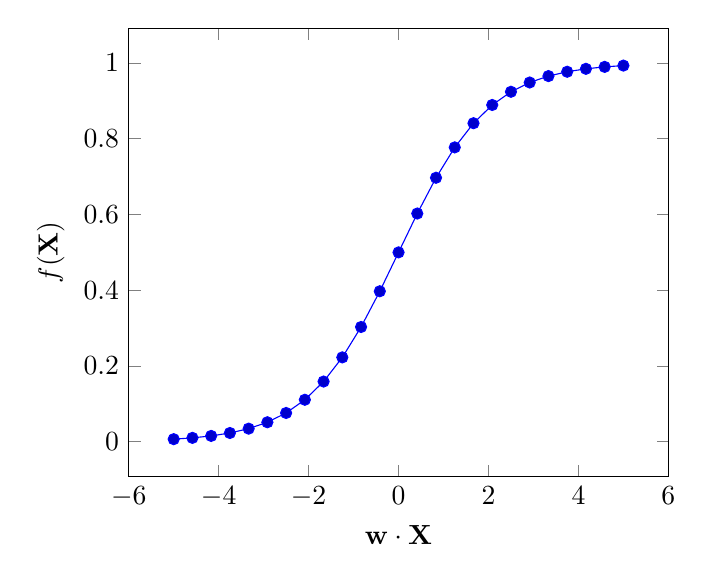
\begin{tikzpicture}
	\begin{axis}[
		xlabel=$\weights\cdot\X$,
		ylabel=$f(\X)$
	]
\addplot {1/(1+ e^-x)}; \end{axis}
\end{tikzpicture}
\end{center}
\end{frame}
\begin{frame}{SGD results}




	Is there a name for this?
\end{frame}

\begin{frame}{Feature weights}
\item["#USER#"]
\end{frame}




\end{document}
